\documentclass[letterpaper,USenglish]{lipics}
\frenchspacing
\interfootnotelinepenalty=10000
%This is a template for producing LIPIcs articles.
%See lipics-manual.pdf for further information.
%for A4 paper format use option "a4paper", for US-letter use option "letterpaper"
%for british hyphenation rules use option "UKenglish", for american hyphenation rules use option "USenglish"
% for section-numbered lemmas etc., use "numberwithinsect"

\usepackage{microtype, xcolor, xspace, cite, units,amsmath,caption}%if unwanted, comment out or use option "draft"
\usepackage{changebar}
% \newcommand{\lsyn}{\lbrack\!\lbrack}
\newcommand{\rsyn}{\rbrack\!\rbrack}
\newcommand{\semp}[1]{\lsyn #1 \rsyn}
%% references
\newcommand{\lnref}[1]{Line~\ref{ln:#1}}
\newcommand{\lemref}[1]{Lemma~\ref{lm:#1}}
\newcommand{\figref}[1]{Fig.~\ref{fi:#1}}
\newcommand{\defref}[1]{Definition~\ref{de:#1}}
\newcommand{\theref}[1]{Theorem~\ref{th:#1}}
\newcommand{\prref}[1]{Proposition~\ref{pr:#1}}
\newcommand{\tabref}[1]{Table~\ref{ta:#1}}
\newcommand{\secref}[1]{Section~\ref{sec:#1}}
\newcommand{\secrefs}[2]{Sections~\ref{sec:#1}--\ref{sec:#2}}
\newcommand{\ssecref}[1]{Sec.~\ref{sec:#1}}
\newcommand{\appref}[1]{Appendix~\ref{sec:#1}}
\newcommand{\exref}[1]{Example~\ref{ex:#1}}
\newcommand{\equref}[1]{eq~(\ref{eq:#1})}
\newcounter{my_counter}
\newcounter{tmy_counter}
\newcommand{\MyRoman}[1]%
        {\setcounter{my_counter}{#1}\roman{my_counter}}
\newcommand{\PMyRoman}[1]%
        {\rm (\MyRoman{#1})}
\newtheorem{MyTheorem}{Theorem}[section]
\newenvironment{The}{%
                \begin{MyTheorem}}{$\QED$\end{MyTheorem}}
\newenvironment{SThe}[1]%
{\par\noindent{\bf Theorem~\ref{The:#1}\/}\begin{em}}%
{\end{em}$\QED$}
\newtheorem{Proposition}[MyTheorem]{Proposition}
\newenvironment{Pro}{%
                \begin{Proposition}}{$\QED$\end{Proposition}}
\newenvironment{SPro}[1]%
{\par\noindent{\bf Proposition~\ref{Pro:#1}\/}\begin{em}}%
{\end{em}$\QED$}
\newtheorem{Lemma}[MyTheorem]{Lemma}
\newenvironment{Lem}{%
                \begin{Lemma}}{$\QED$\end{Lemma}}
\newenvironment{SLem}[1]%
{\par\noindent{\bf Lemma~\ref{Lem:#1}\/}\begin{em}}%
{\end{em}$\QED$}
\newenvironment{Claim}[1]%
{\par\noindent\begin{rm}{\em Claim\/}:~#1}%
{\end{rm}}
\newenvironment{CProof}[1]{\par\noindent %
\begin{rm}{\em Proof of Claim\/}#1:}{\end{rm}}
\newtheorem{Corollary}[MyTheorem]{Corollary}
\newenvironment{Cor}{\begin{Corollary}}{$\QED$\end{Corollary}}
\newtheorem{Conjecture}[MyTheorem]{Conjecture}
\newenvironment{Con}{\begin{Conjecture}}{$\QED$\end{Conjecture}}
\newtheorem{Observation}[MyTheorem]{Observation}
\newenvironment{Obs}{%
                \begin{Observation}}{$\QED$\end{Observation}}
\newtheorem{Definition}[MyTheorem]{Definition}
\newenvironment{Def}{\begin{Definition}}{$\QED$\end{Definition}}
\newtheorem{Example}[MyTheorem]{Example}
\newenvironment{Exa}{\begin{Example}\begin{rm}}%
                        {\end{rm}$\QED$\end{Example}}
\newenvironment{Ex}{\begin{quote}{\bf Example}.}%
                        {$\QED$\end{quote}}
\newenvironment{Note}{\par\noindent{\em Note\/}:}{}
\newenvironment{Remark}{\par\noindent{\bf Remark\/}.}{$\QED$}
\newenvironment{Proof}{\par\noindent %
{\em Proof:\/}\begin{rm}}{\end{rm}}
\newenvironment{ProofA}{%
\begin{rm}{\em Proof:\/}}{\end{rm}}
\newenvironment{ProofW}{\newline %
\begin{rm}{\em Proof:\/}}{\end{rm}}
\newenvironment{ProofIfA}{%
\begin{rm}{\em Proof of the if direction:\/}}{\end{rm}}
\newenvironment{ProofIf}{\newline %
\begin{rm}{\em Proof of the if direction:\/}}{\end{rm}}
\newenvironment{ProofOnlyIfA}{%
\begin{rm}{\em Proof of the only-if direction:\/}}{\end{rm}}
\newenvironment{ProofOnlyIf}{\newline %
\begin{rm}{\em Proof of the only-if direction:\/}}{\end{rm}}
\newenvironment{Sketch}{\par\noindent %
\begin{rm}{\em Sketch of Proof:\/}}{\end{rm}}
\newenvironment{Name}{\begin{bf}(}{)\end{bf}}
\newenvironment{Basis}{\newline {\em Basis\/}:}{}
\newenvironment{Hypothesis}{\newline {\em Induction hypothesis\/}:}{}
\newenvironment{Step}{\newline {\em Induction step\/}:}{}
\newenvironment{CSD}%

\newcommand\numberthis{\addtocounter{equation}{1}\tag{\theequation}}
\newcommand{\eat}[1]{}
\newcommand{\allnotes}[1]{}
% To make the FIXMEs go away, comment out this line...
%\renewcommand{\allnotes}[1]{\textit{#1}}
\newcommand{\fixme}[1]{\allnotes{\bf\textcolor{red}{[#1]}}}
\newcommand{\notescott}[1]{\allnotes{\textcolor{blue}{[Scott: #1]}}}
\newcommand{\noteori}[1]{\allnotes{\textcolor{green}{[Ori: #1]}}}
\newcommand{\notemooly}[1]{\allnotes{\textcolor{purple}{[Mooly: #1]}}}
\newcommand{\notekaterina}[1]{\allnotes{\textcolor{gray}{[Katerina: #1]}}}
\newcommand{\notepanda}[1]{\allnotes{\textcolor{cyan}{[Panda: #1]}}}
\newcommand{\eg}{{\it e.g.,}\xspace}
\newcommand{\ie}{{\it i.e.,}\xspace}

\bibliographystyle{plain}% the recommended bibstyle

% Author macros::begin %%%%%%%%%%%%%%%%%%%%%%%%%%%%%%%%%%%%%%%%%%%%%%%%
\title{New Directions for Network Verification}
\author[1]{Aurojit Panda}
\author[2]{Katerina Argyraki}
\author[3]{Mooly Sagiv}
\author[4]{Michael Schapira}
\author[5]{Scott Shenker}
\affil[1]{UC Berkeley}
\affil[2]{EPFL}
\affil[3]{Tel Aviv University}
\affil[4]{Hebrew University of Jerusalem}
\affil[5]{UC Berkeley and ICSI}
\authorrunning{A. Panda, K. Argyraki, M. Sagiv, M. Schapira, S. Shenker}
\Copyright{Aurojit Panda, Katerina Argyraki, Mooly Sagiv, Michael Schapira and Scott Shenker}
%mandatory, please use full first names. LIPIcs license is "CC-BY";  http://creativecommons.org/licenses/by/3.0/

\subjclass{C.2.6 Internetworking, F.3.1 Specifying and Verifying and Reasoning about Programs}
% mandatory: Please choose ACM 1998 classifications from http://www.acm.org/about/class/ccs98-html . E.g., cite as "F.1.1 Models of Computation".
\keywords{Middleboxes, Network Verification, Stateful Dataplane}% mandatory: Please provide 1-5 keywords
% Author macros::end %%%%%%%%%%%%%%%%%%%%%%%%%%%%%%%%%%%%%%%%%%%%%%%%%

%Editor-only macros:: begin (do not touch as author)%%%%%%%%%%%%%%%%%%%%%%%%%%%%%%%%%%
\serieslogo{}%please provide filename (without suffix)
\volumeinfo%(easychair interface)
  {Billy Editor and Bill Editors}% editors
  {2}% number of editors: 1, 2, ....
  {Conference title on which this volume is based on}% event
  {1}% volume
  {1}% issue
  {1}% starting page number
\EventShortName{}
% \DOI{10.4230/LIPIcs.xxx.yyy.p}% to be completed by the volume editor
% Editor-only macros::end %%%%%%%%%%%%%%%%%%%%%%%%%%%%%%%%%%%%%%%%%%%%%%%

\begin{document}

\maketitle
% \begin{abstract}
% \end{abstract}
\begin{abstract}
Network verification has recently gained popularity in the programming languages and verification community. Much of the recent work in this area has focused on verifying the behavior of simple networks, whose actions are dictated by static, immutable rules configured ahead of time. However, in reality, modern networks contain a variety of middleboxes, whose behavior is affected both by their configuration and by mutable state updated in response to packets received by them. In this position paper we critically review recent progress on network verification, propose some next steps towards a more complete form of network verification, dispel some myths about networks, provide a more formal description of our approach, and end with a discussion of the formal questions posed to this community by the network verification agenda.
\end{abstract}

\section{Introduction}
\label{sec:introduction}

Verification --- by which we mean the general practice of checking the correctness of a computer-based system before it is put into use --- was first developed to
check the correctness of hardware, and is now increasingly used in the software development process. While networks have been around for many decades and are now an essential piece of our computational infrastructure, only recently has verification been applied to ensure their correctness.\footnote{There has been much work on verifying network protocols and their implementations, but until recently almost none on verifying a given network configuration.} As a result, there is now a growing literature on systems that can verify that the current or proposed network configuration (as represented by router forwarding tables) obey various important invariants (such as no routing loops or dead-ends).
These systems --- which allow network operators to verify that their networks will operate correctly, in terms of some well-defined invariants --- represent a valuable, and long overdue, step forward for networking, which for too long was satisfied with not only {\em best-effort} service but also {\em best-guess} configuration. In this position paper we critically review this recent progress, propose some next steps towards a more complete form of network verification, dispel some myths about networks, provide a more formal description of our approach, and end with a discussion of the formal questions posed to this community by the network verification agenda.

In the rest of this section, we provide some necessary background on networks and the current verification techniques. The application of verification to networking coincided with the rise of Software-Defined Networking (SDN). While not essential for the use of verification in networks, SDN provides a useful platform on which to deploy these tools so we discuss verification within the SDN context. Networks are comprised of two planes: the {\em data plane} which decides how packets are handled locally by each router (based on the local forwarding state and other information, such as state generated by previous packets), and the {\em control plane} which is a global process that computes and updates the local forwarding state in each router. In legacy networks, both planes are implemented in routers (with the data plane being the forwarding code or datapath, and the control plane being the global routing algorithm), but in SDN there is a clean separation between the two planes. The SDN control plane is logically centralized, and implemented in a few servers (called controllers) that compute and then install the necessary forwarding state. SDN-controlled routers only implement the data plane, executing a very simple datapath (OpenFlow \cite{openflow}) in which the routing state is a set of
$\langle \textit{match}, \textit{action} \rangle$ flow entries: all packets with headers matching the $match$ entry are subject to the specified $action$ which is often either to forward out a specific port (perhaps with a slightly modified header) or to drop the packet.
One can think of this network state as the {\em configuration} of a router.

The first wave of verification tools \cite{anteater,khurshid2012veriflow,oldhsa,kazemian2013real} analyzed the global behavior of a network made up of switches obeying this simple forwarding model. As a packet travels through the network, its next-hop is dictated by the routing state in the current router; thus, this network-wide behavior can be thought of as the composition of the routing state in each router. These early verification tools would take a snapshot of network state (either that which is already in the network, or that which the control is poised to insert into the network) and then verify whether some basic invariants held. These invariants (which are specified by the network operator) are typically quite simple and few in number: reachability (e.g., packets from host A can reach host B), isolation (e.g., packets from host A cannot reach host B), loop-freedom (no packet enters into an infinite loop), and no dead-ends (no packet arrives at a router which cannot forward it to another router or to the end-destination). Subsequent network verification tools (e.g., \cite{guha2013machine,anderson2014netkat,flowlog, nelson2013balance}) make the same assumptions about the datapath, but generalize along various other dimensions.

All of these tools leverage the fact that the simple forwarding model renders the datapath {\em immutable}; by this we mean that the forwarding behavior does not change until the control plane explicitly alters the routing state (which happens on relatively slow time scales). Thus, one can verify the invariants before each control-plane-initiated change and know that the network will always enforce the operator-specified invariants.

While the notion of an immutable datapath supported by an assemblage of routers makes verification tractable, it does not reflect reality. Modern enterprise networks are comprised of roughly $\nicefrac{2}{3}$ routers\footnote{In this paper we do not distinguish between routers and switches, since they obey similar forwarding models.} and $\nicefrac{1}{3}$ {\em middleboxes}~\cite{sherry2012making}.  Middleboxes --- such as firewalls, WAN optimizers, transcoders, proxies, load Balancers, intrusion detection systems (IDS) and the like --- are the most common way to insert new functionality in the network datapath, and are commonly used to improve network performance and security.\footnote{We should note that the NFV movement is moving middleboxes out of separate physical machines and into VMs that can be hosted on a cluster of servers; however, nothing in the move from physical to virtual middleboxes changes our story.} 

Just as the configuration of a router is the state it uses to make forwarding decisions, the configuration of a middlebox is its set of policies (e.g., drop all Skype packets). The configuration of a network is the configurations of all of its routers, all of its middleboxes, and the topology of the physical network connecting these elements. The goal of verification is to ensure that a given network configuration supports a given invariant.

While useful, middleboxes are a common source of errors in the network~\cite{potharaju2013demystifying}, with middleboxes 
being responsible for over $40\%$ of all major
incidents in networks. Thus, one cannot ignore middleboxes when verifying network configurations.

However, middleboxes do not adhere to the simple forwarding model in routers. Many middleboxes have a {\em mutable} datapath, in which the handling of a packet depends not just on immutable forwarding state, but also on the sequence of previously encountered packets (e.g., a firewall allows packets from a flow into a network, but only if it has previously seen an outgoing packet from that flow).  This dependence on the packet histories renders the datapath quite mutable (changing on packet timescales). This prevents the use of current verification techniques, because the control over packet behaviors is no longer centralized in the control plane, but can depend on the sequence of packets seen by each middlebox.


Thus, we must find a way to verify network behavior in the presence of middleboxes, which means finding verification techniques that can deal with mutable datapaths. Since the forwarding behavior of a mutable datapath can depend arbitrarily on the past packet history, middleboxes render the network Turing-complete. Thus, any verification technique that copes with middleboxes will look much more like general program verification than the current generation of network verification tools. There are two main technical challenges to building the next generation of network verification tools:
\begin{itemize}
\item How do we model these mutable datapaths so that verification is tractable?
\item How can we feasibly analyze a network made up of these mutable datapaths?
\end{itemize}
We address these two challenges in the following sections, and then discuss  how to formalize this approach and end by describing a set of open questions.
\section{How to Model Middleboxes?}
\label{sec:mbmodel}
The natural approach for verifying mutable datapaths would be to apply standard program verification techniques to the code in each middlebox (and then somehow extend this to the network as a whole, which is the problem we address in the next section). The practical problem with this approach is that middlebox code is typically proprietary, and any approach that relies on middlebox vendors releasing their code is doomed to fail.
Moreover, there is a deeper conceptual problem with this approach. The invariants specified by network operators often use abstractions, such as user identity, host identity, application-type (of the traffic), and whether or not the traffic is ``suspicious'' (e.g., after deep packet inspection). In fact, recent efforts to build policy languages are built around a similar set of abstractions~\cite{congress}.

The correctness of these abstractions often {\em cannot} be fundamentally verified (e.g., a middlebox in the middle of the network cannot always know for sure which host the packet came from given the various forms of spoofing or relaying available) or even precisely defined (e.g., what is suspicious traffic?). Yet these abstractions are quite useful (and already widely used) in practice, and operators are willing to live with their approximations (e.g., various techniques can be used to limit spoofing so that in some contexts host identification can use IP or MAC addresses as the basis for identification without great risk).

To allow reasoning in terms of high level abstractions without worrying about the various approximations that go into their definition, we model middleboxes in two parts: a reasonably simple abstract model that captures the action of a middlebox in terms of high-level primitives and an Oracle that is described by the set of abstractions it supports. The Oracle maps packets to one or more abstractions (e.g., this packet is from a Skype flow from host A and user X to host B and user Y), while the abstract model describes how the middlebox uses these abstractions (e.g., a middlebox might be configured to drop all suspicious packets, or only allow packets from host A to reach host B but no other hosts). For instance, for an IDS that identifies suspicious packets and forwards them to a scrubbing box, the Oracle part of the model is what determines which packets are suspicious and the abstract model is what dictates that such packets are forwarded to a scrubbing box.

The Oracles in different middleboxes may use very different techniques to map packets to abstractions. While operators care about the quality of this mapping, the goal of our network verification approach is to check that a network configuration correctly enforces invariants {\em assuming that the Oracles are correct}. Also, different Oracles may  support different sets of abstractions (e.g., some firewalls may be able to identify Skype traffic, and others not), and this would be described as part of the middlebox model.

In contrast, the abstract models are fairly generic in the sense that the abstract model of a firewall applies to most firewalls. The degree of detail in these abstract models depends, to some degree, on the kind of invariants one wants to enforce.  The basic network invariants of reachability and isolation only require that the abstract model describe the forwarding behavior (e.g., if and where each packet is forwarded). These basic invariants of reachability and isolation are our initial target, as these properties are by far the most important use of network verification. If one wants to support performance-oriented invariants then the abstract model must include timing information (e.g., what packet delays might occur), and other extensions are needed to consider invariants that address simultaneity (two properties always hold at the same time). For simplicity, we do not consider such extension here.

Separating middlebox models into an abstract model and an Oracle has several advantages.
\begin{itemize}
\item It captures the fact that there are a limited number of middlebox ``types'', with many implementations of each. The abstract model applies to all of these implementations (and is fairly simple in nature), while the Oracle typically differs between implementations.  Thus, our verification approach --- which asks whether invariants are enforced assuming the Oracles are right --- can be applied independent of the implementations.
\item It differentiates between improvements in the Oracle (e.g., finding better methods for identifying application traffic), which is what consumes the bulk of the development effort, and verifying correctness of the network configuration.
\item It could change the vendor ecosystem by allowing (or requiring) vendors to provide the abstract model (and a description of which abstractions their Oracle supports) along with their middlebox.
Network operators could then perform verification, while vendors could keep their implementations private.
\item While it would be useful for vendors to {\em verify} that their code obeys the abstract model (using standard code verification methods), what makes this approach particularly appealing is that vendors and operators alike can {\em enforce} that the middleboxes obey the abstract model. The abstract models (and we have built several of them) are so simple that they execute much faster than the actual middlebox implementation, so one can run these abstract models in parallel and ensure that the middleboxes take no action that does not obey the abstract model.

\end{itemize}

% \notepanda{The goal is to help network operators verify the correctness of their network configuration before deployment.}
% \notepanda{Configurations and invariants
% are both provided by network administrators.}

\eat{
\begin{lstlisting}[caption={Model for an IDS},label=list:ids,captionpos=t,float,abovecaptionskip=-\medskipamount]
oracle suspicious? (history: Seq[Packet], packet: Packet) : Boolean;


model ids (n: Node, p: Packet) = {
  state history: Seq[Packet];
  when ids_classifier(history, p) =>
      history = history + p;
      forward {p}
  default =>
      history = history + p;
      forward {}
}
\end{lstlisting}

Next we look at the problem of specifying generic middleboxes. For all the middlebox types we have looked at so far, splitting the middlebox into a generic
model and an oracle, allows us to specify the the generic models without loops. This is reasonable since middleboxes must forward packets in bounded time to
keep up with the network and can only touch a bounded amount of state for each packet. }

\section{Network-Wide Verification}
\label{sec:modelnet}

Modeling of individual middleboxes is only the first step; our ultimate goal is to veryify network-wide invariants in a network containing middleboxes and routers.
There are numerous technical challenges (such as how to deal with loops), but in this short position paper we focus on the most challenging one: how can we feasibly perform verification in very large networks (containing on the order of thousands of middleboxes and routers)? To see why this is hard, consider the case of an isolation invariant (packets from host A cannot reach host B) in a network with many middleboxes. Since middlebox behavior depends not just on their configuration but on the packet history they've seen (since their datapath is mutable), verifying that this invariant holds, even if we ignore the possibility of packet loops,
involves checking that there is no sequence of packets --- involving packets sent from anywhere in the network --- which includes a packet from host A reaching host B.


Without additional assumptions, this is not feasible. However, we note that the most common classes of middleboxes have an important property: the handling of a packet from host A to host B depends only on the sequence of packets (seen by the middlebox) between hosts A and B. That is, many mutable datapaths exhibit a useful kind of locality.
For instance, in IP
firewalls, the middlebox tracks established connections, and allows packets to pass if they are either explicitly permitted by
policy or belong to an established connection. A connection between host A and B can only be established by host A and B. We therefore do not need to consider the
actions of any other hosts in the network. We call such middleboxes RONO (Rest-Of-Network Oblivious) middleboxes. RONO is not a rare property; in fact, most middleboxes (including firewalls, WAN optimizers, load balancers, and others) can be configured to be RONO (e.g., caches are RONO if they support ACLS).  Moreover, one can verify whether a middlebox is RONO by statically analyzing its abstract model.


Note that the composition of RONO middleboxes is also RONO.  As a result, in a network containing only RONO
middleboxes we can verify reachability properties on a small subset of the network (the path between two hosts) and these properties would equivalently hold in
the context of the wider network. We have leveraged this fact to verify correctness of a 30,000 middlebox network in under two minutes.


\eat{

RONO middleboxes are not rare in-practice and several non-RONO middleboxes (such as content caches) are extended to make them RONO. Common implementations of
content caches accept ACL rules to limit where content can be accessed from and where correctly configured these act as RONO equivalent middleboxes. One can
statically verify if a model is RONO.

While RONO is one property that allows faster verification of properties in such networks, we believe other properties such as compositionality or commutativity
might also apply to several middleboxes and might enable faster verification. In the next section we talk about some properties that we believe (but have not
proven) hold for stateful dataplane element and help with network verification.

We do not have a general solution for this problem, but have an approach that can scalably verify simple reachability and isolation invariants under certain restrictions.
}
\eat{Now that we have described our models of individual middleboxes, we turn to modelling the network itself. This is harder than reasoning about stateless
networks for a few reasons
\begin{enumerate}
\item When dealing with mutable state, we must account for more than just a single packet. We thus must reason about all paths through the network
      and their effect on state, this might affect both scalability and decidability when verifying properties.
\item Temporal effects become important, in particular the order of packets processed by a middlebox affects its state.
\item Even when dealing with a single packet, network loops might require that we reason about unbounded sequences of data path elements. What makes this worse
      than the stateless case is that every loop through the network might affect the state in the data path. Concretely this means we cannot deal with loops using
      the Kleene star (as is suggested in NetKAT~\cite{anderson2014netkat}), since each iteration cannot be modeled as applying the same policy repeatedly.
      Further, stateful loops imply that the datapath might be Turing complete and verifying any property might easily become undecidable.
\item Even loop free networks can be huge, involving several 10s of thousands of switches, middleboxes, etc. The size is a challenge for scalability.
\end{enumerate}
In this section we present a few techniques we have used to deal with these challenges.

First, we deal with simple forwarding loops, \ie forwarding loops that are caused by static configuration, for instance loops that are obvious from
examining the forwarding tables of switches, by leveraging existing work. To do this, given a network topology with middleboxes, we create an equivalent
topology where the middlebox is replaced by a switch with the same forwarding behavior as the middlebox: \ie the equivalent switch forwards a given packet
the same way the middlebox would if it had output the same packet \notepanda{Fix wording}. We use Veriflow (HSA or other tools could be used as easily) on this
equivalent topology to verify that they are loop-free. Our current tool can only operate on loop-free topologies so we report a verification when this is not
the case. Analyzing static configuration is also more scalable, so we also use the output of these tools (in loop-free toplogies) to eliminate switches: we generate
network transfer functions between all pairs of middleboxes and hosts in a network. We
then derive a network topology where all switches are replaced by a single switch that implements this transfer function. This topology is equivalent to the
original network topology (as has been shown in HSA, VeriFlow, and other works).


Even in this simplified, loop free topology, verifying a property might require analyzing $O(2^n)$ for a network with $n$ middleboxes.
While we do not have a general solution for this problem, we have a specific solution that allows us to verify an important class of properties in networks which
only contain a limited type of middleboxes.
Our solution is applicable to properties which reason about transfers between two hosts (or classes of hosts). Examples of such invariants include:
\begin{itemize}
\item Can host A send packets to host B?
\item Can a host outside the enterprise connect to the mail server?
\item Can host A access data that originated at host B?
\end{itemize}
Note, for stateless data planes, these properties can be checked by traversing all paths between the two hosts (or classes of hosts) and verifying that they hold
(or finding a counterexample). This is not as simple once state comes into play, any communication that goes through the middlebox might affect its behavior and
hence the entire network must be analyzed.
}

\section{Common Myths about Networks and SDN Verification}

We next highlight some common myths about SDN networks and contrast them with the reality of today's networks.

% \medskip{}

\subparagraph*{Myth \#1:} \emph{SDN networks only have controllers and OpenFlow routers, with all complicated (particularly mutable) packet processing done at the controller.} The early SDN literature~\cite{gude2008nox, monsanto2013composing} showed examples where anything expressible using OpenFlow rules was pushed down to routers, while anything more complex was implemented in the controller. Complicated functionality included both complex processing that could not be performed at routers and simple tasks that required mutability (\eg learning switches and stateful firewalls). However, doing this processing at the controller does not scale and, in reality, middleboxes are used to provide most of the processing functions not implementable on routers, and most routers provide some mutable behavior (e.g., learning switch).

\subparagraph*{Myth \#2:} \emph{Centralization, as provided by SDN, is what makes current network verification efforts possible.} Centralization is neither necessary nor sufficient for network verification. {\underline{Not necessary}:} Verification in a network with immutable datapaths only requires being able to access router forwarding state, and current commercial network verification efforts can do this in legacy networks by using commonly available commands to read this forwarding state. {\underline{Not sufficient}:} Regardless of SDN, current network verification efforts cannot verify networks that have middleboxes with mutable datapaths (which describes almost all real networks).


\subparagraph*{Myth \#3:} \emph{Middleboxes are an aberration that will be eliminated by the rise of SDN.} Quite the opposite is true. Not only are middleboxes here to stay, but SDN itself has been evolving to incorporate middleboxes~\cite{scottI2talk}. Furthermore, recently there has been an effort to move middleboxes from dedicated hardware (which is time-consuming to deploy) into virtual machines that can be deployed on quicker timescales, on existing hardware, and at lower cost. This effort is generally described as NFV (network function virtualization), and has gained significant traction commercially (comparable to or exceeding that of SDN), and recent efforts at defining a common configuration language, \eg Congress`\cite{congress}, treat middleboxes (virtualized or not) as first-class network citizens.


\subparagraph*{Myth \#4:} \emph{We should write all network code and configuration in declarative languages, because their use makes verification easy.} In general, reasoning about declarative languages is undecidable~\cite{Halevy}. It is true that verification is easy for declarative programs that do not use recursive rules (e.g., Congress~\cite{congress} or NLOG programs), even in the presence of mutable states. But then, verification is equally easy for imperative programs (e.g., Python, Java, or C programs) that honor certain restrictions, e.g., do not use loops. So, in the end, it is unclear that declarative languages can make a practical difference in verification. Some argue that declarative programs are easier to read and debug, once a programmer gets used to them. On the other hand, their readability becomes questionable in the presence of side-effects.

% \medskip

Once one discards these myths, it becomes clear that network-verification efforts must directly confront the presence of mutable datapaths. While the approach described here may not be optimal, it is currently the only one that confronts the reality of today's and tomorrow's networks. It is time to take the next step in network verification.


\eat{
\begin{outline}
\1 SDN networks only have controllers and OpenFlow routers, with all complicated (particularly mutable [make point about complicated and mutable two different things]) processing done at the controller (e.g., learning switches, firewalls).
    \2 Centralizing it is unscalable, and Middleboxes keep some (all?) mutable processing in the network; an approach already in widespread use
\1 SDN's centralization makes verification possible
    \2 Centralization is neither necessary nor sufficient for verification
    \2 Commercial verification efforts deal with legacy (just read routing state)
    \2 Centralization not sufficient for middleboxes
\1 Middleboxes are an abomination that SDN will eliminate
    \2 Get real: they are widely deployed, essential for security and performance. NFV is outstripping SDN in terms of deployment.
    \2 Instead, SDN will (and already has) evolve to incorporate middleboxes (see Scott's talk)
\1 Write all network code and configuration in declarative languages, since declarative $\implies$ decidable checking of properties
    \2 Not a good way to write middleboxes: Declarative not as useful in the presence of mutable state and side-effects~\cite{Tjgreen}.
        \3 State mutation is imperative in nature and control flow of a program specific ordering and such
        \3 Hard to call out to imperative code, etc. none of the existing work in building middleboxes is easily adaptable.
    \2 Perhaps reasonable for specifying network configuration~\cite{congress} but does not help with verification with mutable datapaths
        \3 Dataplane is Turing complete (as opposed to OpenFlow), controller complexity has nothing to do with undecidability
        \3 Use it if it works for you, not a magic bullet.
\end{outline}
}
% \begin{description}
% \item [Myth] The only options for packet handling are reactive and proactive.
% \item [Reality]  Reactive is usually not an option and proactive may not be powerful enough. Middleboxes compliments the two and is/will be widespread.
% \end{description}

% \begin{description}
% \item [Myth] Centralized solutions can scale well in networks by periodically installing rules.
% \item [Reality] Middleboxes enable scalability while allowing complex distributed functionality using mutable states.
% \end{description}

% \begin{description}
% \item [Myth] SDN opens up the possibility for network verification.
% \item [Reality] The OpenFlow drastically simplifies network verification but it is not realistic and thus any verification effort which can \textbf{only} handles
% OpenFlow has limited applicability.
% \end{description}


% \begin{description}
% \item [Myth] Learning switches and statful firewalls need to be implemented in the controller.
% \item [Reality] Learning switches are some of the simplest and most common dataplane elements and are not normally implemented using a controller. A stateful
% firewall is a very common middlebox.
% \end{description}

% \begin{description}
% \item [Myth] The use of declarative languages renders network verification problems decidable.
% \item [Reality] . Declarative programming languages have been used to effectively express network policies in languages like Nlog~\cite{Nlog},
% Flowlog~\cite{flowlog}, NDLog~\cite{}, NetCore~\cite{monsanto2012compiler} and have also been recently used to describe network configuration~\cite{Congress}.
% However, these languages loose their charm in the presence of side-effects and mutable state~\cite{Tjgreen}.
% State mutation is imperative by nature and the control flow of a program is used to specify how these updates are processed. Specifying state updates
% using a declarative language quickly becomes counterproductive as a result.
% Furthermore, even simple updates result in a Turing complete language~\cite{Janos}, thereby preventing the compiler from handling
% \textbf{all} programs. Further, calling imperative code from declarative programming is challenging and further prevents optimization and runtime checking.
% Finally, we note that these languages lack mechanisms for modularity such as procedures, modules, packages, and classes which are
% heavily used in building middleboxes and complex network code.
% \end{description}

% \begin{description}
% \item [Myth] Middleboxes are abomination
% \item [Reality] Middleboxes are necessity. Half of the network;
% Solving real and pressing problems;
% Needs that are not likely to go away;
% Enable local functionality enhancements~\cite{Riverved}
% \end{description}

\section{Formalizing the Mutable Data Plane}
\label{sec:formal}
The previous sections argued why a new approach to network verification is needed and briefly outlined what it might look like.
In this section, we sketch a concrete way to formalize and prove interesting  properties of networks of middleboxes.

\begin{lstlisting}[caption={Model for an IDS},label=list:ids,captionpos=t,float,abovecaptionskip=-\medskipamount,
                    numbers=left,
                    morekeywords={oracle, model, when, default, state, forward},belowskip=-0.1in]
oracle suspicious? (packet: Packet) : Boolean;

model ids (p: Packet) = {
  when suspicious?(p) =>
      forward {}
  default =>
      forward {p}
}
\end{lstlisting}

% \subsection{Verification Problem}
DeMillo et al.~\cite{popl:DeMilloLP77} previously argued that specifying the desired behavior of a program (or network) is hard. 
Indeed, the lack of a precise specification is a major problem for program and network verification. 

The primary function of networks is to allow hosts to communicate with each other. Reachabality, the property that a certain class of packets sent from host $A$ can reach host $B$, and its converse, isolation, are fundamental to networks: all useful networks must satisfy some set of reachability properties and their verification is thus universally important. In the rest of this section we limit our discussion to Reachability invariants.

We formally state these invariants using temporal logic where we assume fairness, \ie we assume any continuously enabled transition will eventually occur. 
First, we define two relations: $Send(n, p)$ indicating some network entity (node) $n$ sent
a packet $p$ (at some time), and $Recv(n, p)$ indicating node $n$ received packet $p$. Given these relations any reachability property can be expressed in
LTL (Linear Temporal Logic) as
\begin{align*}
\forall p\in \text{Packet}: \Box (Send(src, p) \land Predicate(p) \implies \Diamond(Recv(dest, p)))
\end{align*}
This temporal logic statement says that a packet $p$ sent by $src$ which satisfies $Predicate$ is eventually received by $dest$.
Similarly, isolation can be formally expressed by requiring that a packet sent by $src$, satisfying $Predicate$ is never received by $dest$:
\begin{align*}
\forall p\in \text{Packet}: \Box (Send(src, p) \land Predicate(p) \implies \Box(\neg Recv(dest, p)))
\end{align*}

$Predicate$ in the definitions above is specified using the same abstractions used to specify network policies, \ie either in terms of packet
header fields (source, destination, etc.) or in terms of the abstraction provided by a middlebox Oracle (\S\ref{sec:mbmodel}). For example, a property
saying no SSH traffic can reach a server $d$ can be expressed as
\begin{align}
\forall s\in \text{Node}, p\in \text{Packet}: \Box (Send(s, p) \land ssh(p) \implies \Box(\neg Recv(d, p))) \label{eq:isossh}
\end{align}

where $ssh(p)$ returns true if an Oracle classifies the packet as belonging to an SSH connection.
We reason about reachability and isolation properties assuming that the Oracles are correct.
Verifying the isolation property in Equation~(\ref{eq:isossh}) therefore requires answering the question:
``assuming SSH traffic is correctly identified, can a packet belonging to an SSH connection reach $d$?''

% \subsection{Formalizing Middlebox Semantics}

% \notepanda{I think we should cut this bit, or move it elsewhere}
As stated earlier, we model a middlebox as an oracle and a simple abstract model. The Oracle provides abstractions that are used to specify the
properties being checked. We expect models for middleboxes (which include both an oracle and a generic model) to be specified
using a constrained programming language. Listing~\ref{list:ids} shows an example of such a specification
for an intrusion detecion system (IDS). The IDS oracle provides one abstraction, \texttt{suspicious?}, defined in the first line. The abstract model is
defined in Lines 4 -- 9 and uses this abstraction. First we check to see if the packet is suspicious (the Oracle's decision here might be based on what
packets it has seen previously), and  drop the packet (Line 6) or forward the packet (Line 9) depending on the value returned by the Oracle.
% \notepanda{End of where we would cut until}

Next, we develop abstract semantics for middleboxes. We use these to reason about general properties (such as composition) that apply to all middleboxes. Our semantic model is defined over a potentially infinite set of packets, $P$.  We augment packets to include information about their location (\ie the
middlebox or
switch port). We also define the operator $\doteq$, such that $p_1 \doteq p_2$ implies that packets $p_1$ and $p_2$ are identical except for their location.
Finally, we use $P^*$ to represent the set of all (potentially unbounded) sequence of packets.
The abstract model middlebox $m$, is then a function $m\colon P\times P^* \to 2^P$ which takes a packet ($p\in P$) and a history ($h\in P^*$) 
of all the packets that have
previously been processed by $m$ and produces a (possibly empty) set of packets $m(p, h)$. Given this model a switch is a simple function for which
$m(p, h) \doteq \left\{p\right\}$. Similarly a simple firewall, $f$ (whose decision process is represented by $allowed$) can be expressed as
\begin{align*}
 f(p, h) = \begin{cases}
    \left\{p'\right\}\ p' \doteq p & \mbox{if } allowed(p, h)\\
    \left\{\right\} & otherwise
 \end{cases}
\end{align*}

% \subsection{Composing Middleboxes}
Ideally, we would like to be able to reason about the network \emph{compositionally}, \ie the correctness of the network should follow from
the correctness of smaller, simpler components. Compositional reasoning can reduce the cost of verification and enable incremental verification
of changes in the network. Compositionality has been important for making verification tractable in other domains, for instance the use of
rely-guarantees~\cite{tse:MisraC81,ifip:Jones83}, was important for enabling verification of concurrent programs.

We start by defining what it means to be able to compositionally verify a network. Let us
define the union of two networks $N_1$ and $N_2$ in the natural way, \ie $N_1\cup N_2$ contains the union of all nodesand links in each of $N_1$ and $N_2$.
Consider two networks: $N_1$, where property $P_1$ holds (represented as $N_1\models P_1$); and $N_2$, where property $P_2$ holds. We can compose the proofs
for properties $P_1$ and $P_2$ if and only if  both $P_1$ and $P_2$ hold for $N_1 \cup N_2$. More formally, we can verify properties $P_1$ and $P_2$
compositionally for network $N$ if for any $N_1 \subset N$ and $N_2\subset N$
\begin{align*}
N_1 \models P_1,  N_2\models P_2\\
\hline
(N_1 \cup N_2) \models P_1\land P_2
\end{align*}

\begin{figure}
\centering
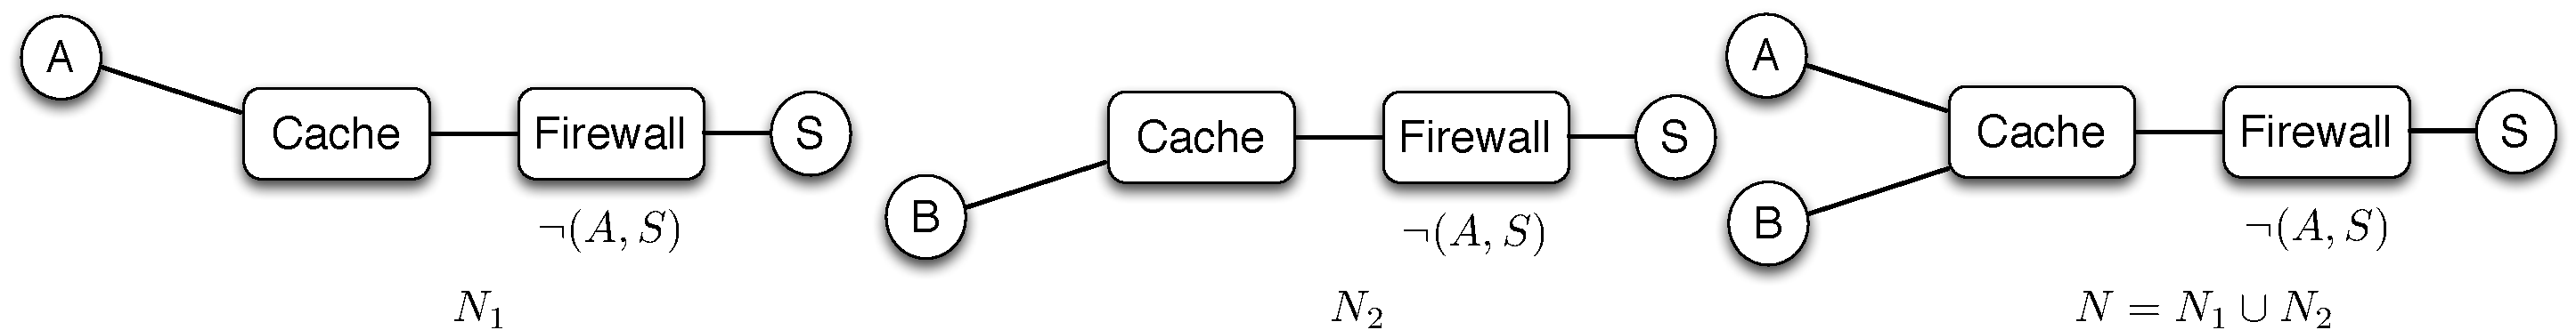
\includegraphics[width=0.9\textwidth]{figures/rono_example.pdf}
\caption{Example where networks are not composable with respect to reachability properties.}
\label{fig:compose_fail}
\vspace{-0.15in}
\end{figure}

Generally, one cannot perform compositional verification of reachability properties. For instance,
consider the example in Figure~\ref{fig:compose_fail}. The cache in this example records all requests to and the corresponding responses from $S$.
On receiving a new request,  the cache checks to see if it has previously recorded a response for this request, in which case it returns the saved response;
otherwise the cached forwards the request, unmodified, to the firewall.
 The firewall drops all requests sent from $A$ to $S$, but otherwise forwards all other requests and responses unmodified.
In network $N_1$, $A$ can never receive a response from $S$ (thus is isolated). However in the composed network $N_1\cup N_2$, if $B$ sends a request $r$ and
receives response $r'$ from $S$, then $A$ can also request $r$ and receive $r'$.

One key insight is that despite being impossible in general, there exists an important subset of networks where compositional reasoning can be used
to verify reachability properties. These networks contain only Rest-Of
Network Oblivious middleboxes (\S\ref{sec:modelnet}), middleboxes whose behavior for a pair of hosts depends only on the traffic sent between these hosts.
More formally, we define the restriction $h|_{(A, B)}$ of a packet history $h\in P^*$ to be the subsequence of $h$ containing only those packets that were
sent between host $A$ and $B$. We define a middlebox $m$ to be RONO if and only if
\begin{align*}
\forall p: p.src = A \land p.dest = B &\ \  f(p, h) = f(p, h|_{(A, B)}) \text{   and}\\
\forall p: p.src = B \land p.dest = A &\ \ f(p, h) = f(p, h|_{(A, B)})
\end{align*}

Not all compositions of RONO middleboxes are themselves RONO. In~\cite{corr:PandaLASS14}, we have identified conditions where a network of RONO middleboxes
supports compositional verification.\fixme{Should include information about RONO and eRONO, and also show an example where pure RONO composition fails.}

\section{Some Open Problems in Network Verification}
%\notepanda{We should consider changing the section title, Open Problems sounds very lofty.}
Finally, we present some open problems that we have encountered while looking at how to verify mutable dataplanes. This list is not 
exhaustive, but is rather an attempt to list the first set of hurdles that need to be crossed given this new network verification agenda.

\subparagraph*{Decidability of Verification} When processing a packet, a middlebox might access potentially unbounded state. This prevents the use
of finite-state model checking, and other verification techniques are undecidable for general programs in this class. We are
currently working on a limited programming language that is rich enough to specify many existing middleboxes and to enable verification of some interesting network properties, including reachability properties. What other network properties can be verified in a decidable manner remains an important open problem.

\subparagraph*{Specification} While we have provided some tools
that allow us to specify and check reachability properties; extending this to other invariants, for example performance-based
invariants is challenging. How middleboxes and properties are specified also has a huge impact on verification time and
decidability. Therefore, it is crucial to pick specifications that are rich enough to permit operators to express interesting and
useful properties, yet narrow enough to permit automated reasoning.

\cbstart
\subparagraph*{Conditions for Compositional Verification} We have found a set of sufficient conditions that allow compositional verification of networks, however
finding a set of necessary conditions remains an open problem. Necessary conditions allowing compositional verification are useful not just for the formal verification community, but might also provide important insights about how networks should be designed and configured.
\cbend

\subparagraph*{Correctness-Preserving Transformations} It might be possible to extend some of our results on compositional reasoning to show that the addition of certain types of middleboxes
can never affect some class of invariants. We know this is true for some middleboxes in reality, e.g., the addition of a stateless firewall
can never affect an isolation invariant (though it might invalidate some reachability invariants). Developing a theory for when this 
holds might be useful in developing techniques to help simplify network changes. 

\subparagraph*{Verifying Parametric Topologies} Some network topologies are parametric. For example, one can generate a fat-tree topology~\cite{al2008scalable} for a given datacenter size. It is possible that we can leverage compositional verification techniques to verify properties independent of the parameter. This would both speed-up verification and perhaps provide insights into the kinds of networks that are easily evolvable.
\section{Acknowledgments}
\label{sec:ack}
\bibliography{snapl}
\end{document}
